\newpage
\part{PyWPS}

\newpage
\section{PyWPS}
\label{sec:PyWPS}
\subsection{History}
The origin of PyWPS started in 2006 as a student project. The first presentation was held at the FOSS4G 2006 conference in Lausanne titled 
‘GRASS goes to web: PyWPS’. During November 2006 the version 1.0.0 was released together with WUIW and Embrio projects that brought the
funcionality of GRASS GIS and general web interface able to handle any WPS server.\cite{PyWPS_presentation}\cite{PyWPS_web}

In 2007 PyWPS 2.0.0 was released supporting WPS standard 0.4.0. New version improved stability a approached on the standard implementation. It came with new WPS client and WPS plugin for OpenLayers \footnote{\url{http://openlayers.org/}}.

Next year in 2008 PyWPS 3.0.0 was released with support for WPS 1.0.0. It was possible to run multiple WPS instances
with one PyWPS installation. This version had simple code structure and contained examples of processes. 

The newest version is PyWPS 4.0.0 from 2016 when PyWPS-4 branch was merged to official PyWPS repository as its master branch.
 New version is described in following Sec. \ref{sec:PyWPS4}.

\begin{figure}[h!]
\centering

\includegraphics[width=0.4\textwidth]{img/pywps_logo.png}
\caption{PyWPS project logo}
\label{fig:pywps_logo}
\end{figure}

\subsection{PyWPS 4.0}
\label{sec:PyWPS4}
PyWPS-4 is the most current version of PyWPS. Rewriting from scratch involved this major changes:
\begin{itemize}
\item It is written in \textit{Python 3} with backward support for Python 2.7.
\item It utilizes native Python bindings to existing projects (GRASS GIS).
\item New popular formats like \textit{GeoJSON}, \textit{KML} or \textit{TopoJSON} are reflected and their support is provided.
\item PyWPS project has changed the license from \textit{GNU/GPL} to \textit{MIT}.
\item PyWPS 4.0 is implemented using the \textit{Flask} framework.
\item A C-based XML parser \textit{Lxml} is used to handle XML files.
\item \textit{OWSLib} structures are used for some data types.
\end{itemize}

\subsection{PyWPS-demo}
\label{sub:demo}
PyWPS-demo is a small side project distributed with PyWPS. It is a simple demo instance of PyWPS server running on 
\textit{Flask}\footnote{\url{http://flask.pocoo.org/}}. Flask is a microframework for web applications in Python. 
Flask provides built-in development server and debugger and RESTful request dispatching. Starting PyWPS-demo server with Flask
is very simple and can be done with command in Lst. \ref{lst:demo_start}. After starting the PyWPS-demo server the PyWPS homepage can be 
visited at: \url{http://localhost:5000}

\bigskip
\begin{lstlisting}[basicstyle=\small,caption={Starting PyWPS-demo server},label={lst:demo_start}]
python3 demo.py
\end{lstlisting}

PyWPS-demo comes with several demo processes:
\begin{itemize}
\item \textit{area.py} - Process calculates area of given polygon.
\item \textit{bboxinout.py} - Process transforms bounding box to another EPSG.
\item \textit{buffer.py} - Process returns buffers around the input features, using the GDAL library.
\item \textit{centroids.py} - Process returns a GeoJSON with centroids of features from  an uploaded GML.
\item \textit{feature\_count.py} - Process counts the number of features in an uploaded GML.
\item \textit{grassbuffer.py} - Process uses the  GRASS GIS \textit{v.buffer} module to generate buffers around inputs.
\item \textit{sayhello.py} - Process returns a literal string output with Hello plus the inputed name.
\item \textit{sleep.py} - Process will sleep for a given delay or 10 seconds if not a valid value.
\item \textit{ultimate\_question.py} - The process gives the answer to the ultimate question of "What is the meaning of life?"
\end{itemize}

Except these example processes the demo offers also example configuration file. Configuration file contains several parameters in
these four sections:
\begin{itemize}
\item \textit{metadata} - parameters containing information for metadata creation.
\item \textit{server} - definition of path to workdir and output directories, maximum number of parallel running or stored processes. 
\item \textit{logging} - logging level setting, path to log file and log database.
\item \textit{grass} - GRASS setting.
\end{itemize}



\newpage
\section{Process isolation in PyWPS}
\subsection{Asynchonous requests}
Right now in PyWPS 4.0 version a PyWPS server instance is able to run multiple
concurrent processes in parallel. The server is configured for maximal amounts of concurrently running processes at
the same time and for the maximal amount of waiting processes in a queue, to later start their execution once new
slots are available. If the new Execute request is received and the maximal amount is exceeded, the request is rejected
and user is informed in response (see Lst. \ref{lst:Isolation_rejected}).

\begin{lstlisting}[basicstyle=\small,caption={Resource exceeded exception},label={lst:Isolation_rejected}]
<?xml version="1.0" encoding="UTF-8"?>
<ows:ExceptionReport xmlns:ows="http://www.opengis.net/ows/1.1" version="1.0.0">
    <ows:Exception exceptionCode="ServerBusy">
        <ows:ExceptionText>
            Maximum number of parallel running processes reached. Please try later.
        </ows:ExceptionText>
    </ows:Exception>
</ows:ExceptionReport>
\end{lstlisting}

To facilitate the management of concurrent processes, process metadata are stored into a local database. This database is used
for logging and saving waiting Execute requests in the queue and invoking them later on.
This database will also enable the implementation of pausing, releasing and deleting running process. These features will
allow PyWPS to comply with WPS version 2.0.0.

\subsection{Current state}
\label{subsec:current_state}
At the beginning of every process execution its own temporary directory \textit{workdir} is created. During the execution
temporary files and continuous outputs are stored in this folder. After successful execution final outputs are
moved to \textit{outputs} directory. Both directories \textit{outputs} and \textit{workdir} are configurable and user can
change path to them.

\bigskip
\begin{lstlisting}[basicstyle=\small,caption={pywps.cfg - mode parameter}]
[processing]
mode=multiprocessing
\end{lstlisting}

Current version of PyWPS offers two solutions for running parallel processes:
\begin{itemize}
\item Multiprocessing
\item Job Scheduler Extension\footnote{Job Scheduler Extension is currently only in develop branch of PyWPS.}
\end{itemize}

If the execute request is sent asynchronously the type of process constructor is chosen depending on configuration
parameter \textit{mode} in section \textit{processing} which is by default \textit{multiprocessing} or can be changed 
to \textit{scheduler}.

\bigskip
\begin{lstlisting}[basicstyle=\small,caption={processing.\_\_init\_\_.py},label={lst:Process_init},language=python]
def Process(process, wps_request, wps_response):
    """
    Factory method (looking like a class) to return the
    configured processing class.

    :return: instance of :class:`pywps.processing.Processing`
    """
    mode = config.get_config_value("processing", "mode")
    LOGGER.info("Processing mode: %s", mode)
    if mode == SCHEDULER:
        process = Scheduler(process, wps_request, wps_response)
    else:
        process = MultiProcessing(process, wps_request, wps_response)
    return process
\end{lstlisting}
\bigskip
\bigskip

\paragraph{Multiprocessing}
By default for  processes   running   in   the   background,   the   Python \textit{multiprocessing} module is used – 
this makes it possible to use PyWPS on the Windows operating system too.

\begin{figure}[h!]
\centering
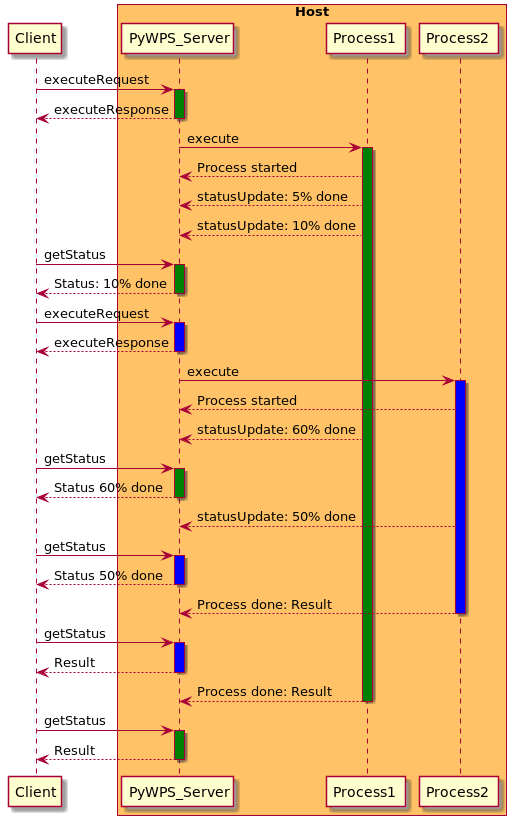
\includegraphics[width=0.7\textwidth]{img/Diag_multiprocessing.png}
\caption{Sequence diagram: Multiprocessing}
\label{fig:Diag_multiprocessing}
\end{figure}

The number of processes running in parallel is configirable by parameter \textit{parallelprocesses} of section \textit{server} in 
configuration file. In the Fig. \ref{fig:Diag_multiprocessing} are shown two running processes. A client sends an Execute request to
a server. Server sends back to the client an ExecuteResponse that \textit{Process1} (green in the figure) was accepted and starts its 
execution. During the execution the process updates its status. The interval of status updates depends on the code of the Process1.
Process1 must support status update otherwise it cannot be run in asynchronous mode.

During the execution of Process1 server receives another Execution request. It sends back the Execution response and starts the execution
of \textit{Process2} (blue in the figure). Separated Python \textit{Process}\footnote{Explanation of term Python \textit{Process} and its
differences to \textit{Thread} is in next paragraph.} is created. Both of the processes run on the host machine but both have own memory
space. Their executions run concurently and client can request their status. In the figure, the Process2 ended first and client can retrieve
the result from the server. Once the Process1 ends too, the client can retrieve its result from the server as well.

It is important to say that in case of multiprocessing processes run concurently with its own memory space nevertheless they are not isolated.
They run on the same host machine and share the resources. There are even methods like \textit{Pipe()} that enables communication between 
processes.

\paragraph{Process vs Thread} In Python there are two ways to achieve \textit{pararellism}. It is \textit{multiprocessing}
\footnote{\url{https://docs.python.org/3/library/multiprocessing.html}} with using processes and \textit{threading}\footnote{https://docs.python.org/3/library/threading.html} with threads. The main difference is that threads run in the same memory space, while processes
have separate memory. Multiprocessing takes advantages of multiple CPUs and cores while threads are more lightweighted and have low memory
footprint. In case of PyWPS asynchronous requests, for every execution its own process with its own memory space is created.

\paragraph{Job Scheduler Extension}
PyWPS scheduler extension offers possibilities to execute asynchronous processes out of the WPS server machine.
This extension enables to delegate execution of processes to a scheduler system like \textit{Slurm}, \textit{Grid Engine} 
and \textit{TORQUE} from Adaptive Computing. These schedular systems are usually located at \textit{High Performance Compute (HPC)}
centers.

\begin{figure}[h!]
\centering
\begin{floatrow}
\ffigbox{
\includegraphics[width=0.33\textwidth]{img/Isolation_grid.jpg}}{\caption{Grid Engine}}{\label{fig:Isolation_grid}}
\ffigbox{
\includegraphics[width=0.25\textwidth]{img/Isolation_slurm.png}}{\caption{Slurm}}{\label{fig:Isolation_slurm}}
\end{floatrow}
\end{figure}

\begin{figure}[h!]
\centering

\includegraphics[width=0.33\textwidth]{img/Isolation_torque.png}
\caption{TORQUE}
\label{fig:Isolation_torque}
\end{figure}
\bigskip

The PyWPS scheduler extension uses the Python \textit{dill} library to dump and load the processing job to/from filesystem. The batch script executed on the scheduler system calls the PyWPS \textit{joblauncher} script with the dumped job status and executes the job (no WPS service running on scheduler). The job status is updated on the filesystem. Both the PyWPS service and the joblauncher script use the same PyWPS configuration. The scheduler assumes that the PyWPS server has a shared filesystem with the scheduler system so that XML status documents and WPS outputs can be found at the same file location. The interaction diagram how the communication between PyWPS and the scheduler works is displayed in Fig. \ref{fig:Isolation_interaction}.

\bigskip
\begin{figure}[h!]
\centering
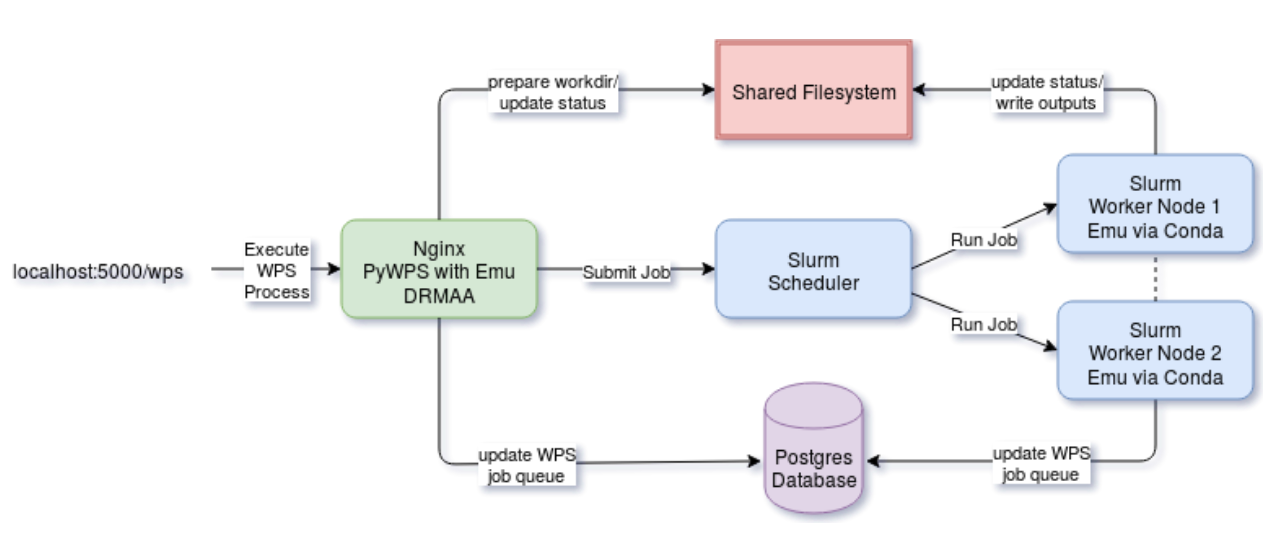
\includegraphics[width=\textwidth]{img/Isolation_slurm_usage.png}
\caption{Example of PyWPS scheduler extension usage with Slurm, source: \cite{PyWPS_docs}}
\label{fig:Isolation_slurm_usage}
\end{figure}

\begin{figure}[h!]
\centering
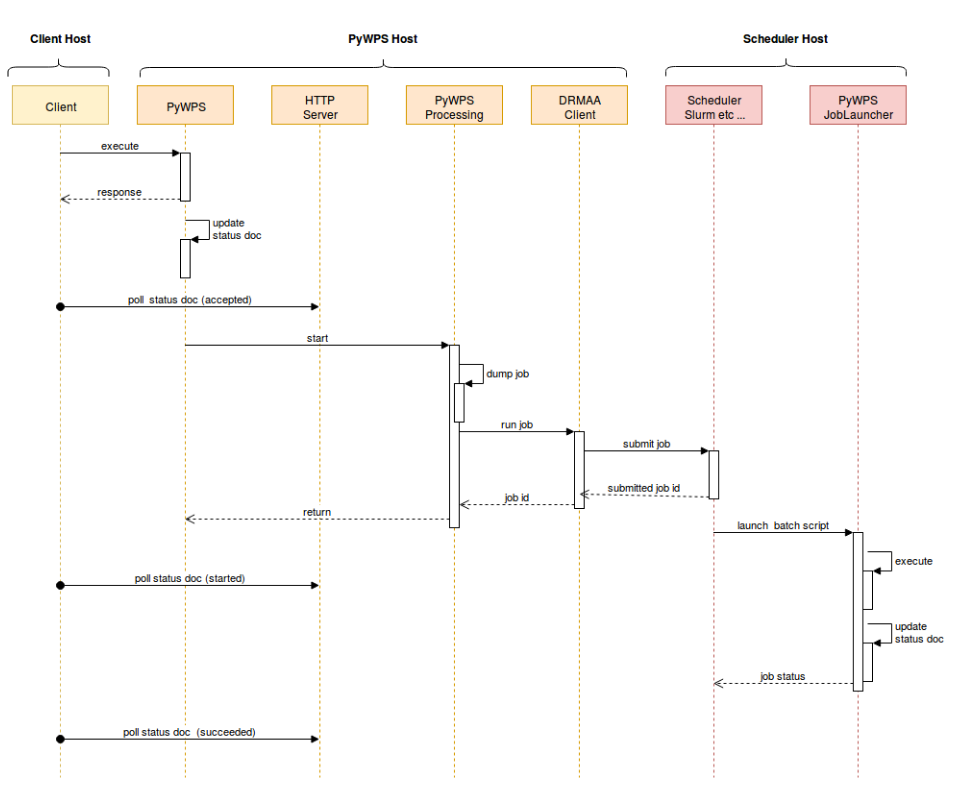
\includegraphics[width=\textwidth]{img/Isolation_interaction.png}
\caption{Communication between PyWPS and scheduler, source: \cite{PyWPS_docs}}
\label{fig:Isolation_interaction}
\end{figure}

\subsection{Possible solutions}
In previous section there were described two mechanisms for running parallel processes. Nevertheless in case of Python module
\textit{Multiprocessing} the processes are not really isolated. They run concurrently but they can share resources and there are 
even methods like \textit{Pipe()} that enables communication between processes.

On the otherhand \textit{Job Scheduler Extension} is dependent on \textit{dill} library as well as on some external scheduler
systems like \textit{Slurm}, \textit{Grid Engine} or \textit{TORQUE}.

\bigskip
In this section there are described some other solutions. Some of them were suggested by PyPWS developers with encouragement to
make a feasible study. Some of them were discovered during research on the internet forums like StackOverflow, some of them
were referenced in the documentation of other projects. During the research two requirements were considered.

\begin{itemize}
\item The solution provides a mechanism for full isolation. This is a must-have requirement.
\item The solution provides a mechanism for start/pause/stop process execution. This is a nice-to-have requirement as this functionality
will be required to comply WPS 2.0.0 standard.
\end{itemize}

\noindent
Finnaly these solutions were considered:
\begin{itemize}
\item Celery
\item Docker
\item psutil
\item SandboxedPython
\item VM
\end{itemize}

\subsubsection{Celery}
\textit{Celery} is a task queue system written in Python. It helps distribute work across threads and even machines. Basic term is
a \textit{task}. A task is a unit of work and it is an input into the task queue. The task queue is constantly monitored for new 
work to perform.

To communicate between client and workers Celery uses a \textit{broker}. The communication is via messages. To initiate a task the
client adds a message to the queue and the broker then delivers the message to a worker. Multiple workers and brokers can be added
so there is assured high availability and horizontal scaling.

Celery provide worker remote control client in class \textit{celery.app.control.Control(app=None)}. The class offers these functions:
\begin{itemize}
\item\textbf{revoke} - Tell all (or specific) workers to revoke a task by id. If a task is revoked, the workers will ignore the task and not execute it after all.
\item\textbf{shutdown} - Shutdown worker(s).
\item\textbf{terminate} - Tell all (or specific) workers to terminate a task by id.
\end{itemize}

\subsubsection{Docker}
\textit{Docker} is one of the most used technology regarding containerization. This technology is described in depth in a later chapter.

\subsubsection{psutil}
\textit{psutil} is Python library for process and system management. It handles system monitoring, limiting process resources
and the management of running processes. Its implementation is based on UNIX command line tools. psutil offers functions applied
to these sections:
\begin{itemize}
\item CPU - functions for CPU statistics such as CPU utilization percentage, frequency and others. 
\item Memory - functions for system memory usage and swap memory statistics.
\item Disks - functions for disk statistics such as disk usage or disk IO operations counter.
\item Network - functions for network IO operations or network connection statistics.
\item Sensors - functions for statistics about fans, battery or hardware temperature.
\item Others - functions for boot time and users statistics.
\item Processes - functions will be described in detail later.
\end{itemize}

\paragraph{Processes} - Class \textit{psutil.Process(pid=None)} represents an OS process with given pid. The class is
bound with a process via its PID. The \textit{Process} class offers these methods for starting/pausing:
\begin{itemize}
\item suspend() - The method suspends a process using SIGSTOP signal.
\item resume() - The method resumes a process using SIGCONT signal.
\item terminate() - The method terminates a process using SIGTERM signal.
\item kill() - The method kills a process using SIGKILL signal.
\end{itemize}

\subsubsection{Sandboxed Python}
The general goal of a sandbox is to run applications securely inside isolated environment they cannot escape from and
affect other parts of the system. Developers use them to run untrusted code inside. It is quite difficult to develop
fully sandboxed solution due to Python complexity. The basic problem is that Python introspection allows several ways
to escape out of the sandbox. True security requires an overall design with many security considerations included. Some
of the projects that can run Python code in a sandbox are:
\begin{itemize}
\item PyPy
\item Jython
\end{itemize}

\paragraph{PyPy} PyPy is Python interpreter written in RPython that implements full Python language and very closely 
emulates the behavior of CPython. PyPy offers fully portable sandboxing feature similar to OS-level sandboxing (e. g. SECCOMP).
It is not sandboxing at the Python language level so it does not put any restriction on any Python functionality.

Untrusted Python code that is intended to be sandboxed is launched in a subprocess, that is a special sandboxed version of PyPy.
All its inputs/outputs are not directly performed but are serialized to a stdin/stdout pipe. The outer process reads the pipe 
and afterward decides which commands are allowed.

\paragraph{Jython} Jython is Python language interpreter for Java. Java offers strong sandboxing mechanisms. The security 
facility in Java that supports sandboxing is the \textit{java.lang.SecurityManager}. By default, Java runs without a 
SecurityManager.

\paragraph{pysandbox} A prove, that it is very difficult to develop some kind of sandbox with all security holes considered, could be a project  \textit{pysandbox}\footnote{\url{https://github.com/vstinner/pysandbox}}. After working on it for 3 years, during which
the project was used on various production servers by other developers, its author declared that the project is broken by
design. In his post to the python-dev mailing list \cite{PyDev_ML} the author explained that with every vulnerability founded
it became more difficult to actually write a real code:

\textit{
"To protect the untrusted namespace, pysandbox installs a lot of
different protections. Because of all these protections, it becomes
hard to write Python code. Basic features like "del dict[key]" are
denied. Passing an object to a sandbox is not possible to sandbox,
pysandbox is unable to proxify arbitary objects.}

\textit{
For something more complex than evaluating "1+(2*3)", pysandbox cannot
be used in practice, because of all these protections. Individual
protections cannot be disabled, all protections are required to get a
secure sandbox."}

\subsubsection{Virtual Machine/Vagrant}
Using full virtualization for process isolation is mentioned here but in fact it is hard to imagine this solution could work
in practice. \textit{Vagrant} is a tool for managing and building virtual machines. It provides a way how to manage various virtual 
machines in an automatized way e. g. using scripts. There also exists a Python package \textit{python-vagrant} that offers 
Python bindings for interacting with Vagrant.

However in our use-case using Vagrant would mean that for every process execution a separate virtual machine is created. Depending
on the process algorithm complexity the process execution can last from milliseconds to hours or days. On the other hand building 
a virtual machine and booting into it last at least few seconds. That is why it is hard to imagine using virtual machine, which takes
few seconds to boot up, to isolate process, which execution lasts less than a second.

\newpage
\section{Docker}
\textbf{Containerization} is a lightweight alternative to full machine virtualization. It involves encapsulating an application 
into a container with its own operating environment. It helps to run a containerized application on any physical machine without any
worries about dependencies. The origin of containerization lies in the \textit{LinuX Containers {LXC}} format. Containerization
works only in Linux environments and can run only Linux applications.

\begin{figure}[h!]
\centering

\includegraphics[width=0.33\textwidth]{img/Docker_logo}
\caption{Docker logo}
\label{fig:Docker_logo}
\end{figure}

Docker is not the only one technology for containerization. Other alternatives exist, it is \textit{Kubernets}, \textit{CoreOS rkt}, 
\textit{Open Container Initiative (OCI)}, \textit{Canonical's LXD}, \textit{Apache Mesos and Mesosphere} and many others. 
However Docker is a leader on the field of containerization and with most public traction is de facto considered as a container standard.
That's why the Docker was chosen for this thesis as a container technology. So from this point on any term \textit{container} refers to
Docker container.

\begin{figure}[h!]
\centering
\begin{floatrow}
\ffigbox{
\includegraphics[width=0.2\textwidth]{img/Docker_kubernetes.png}}{\caption{Kubernetes}\label{fig:Docker_kubernetes}}
\ffigbox{
\includegraphics[width=0.2\textwidth]{img/Docker_rkt.png}}{\caption{CoreOS rkt}\label{fig:Docker_rkt}}
\end{floatrow}
\end{figure}

\begin{figure}[h!]
\centering
\begin{floatrow}
\ffigbox{
\includegraphics[width=0.13\textwidth]{img/Docker_lxd.png}}{\caption{Canonical's LXD}\label{fig:Docker_lxd}}
\ffigbox{
\includegraphics[width=0.25\textwidth]{img/Docker_mesos.jpg}}{\caption{Apache mesos}\label{fig:Docker_mesos}}
\end{floatrow}
\end{figure}

\paragraph{Docker} is a Linux container technology that allows package and ship applications and everything it needs to execute into a standard
format, and run them on any infrastructure.

\subsection{Virtual machine vs. Docker container}
Both virtual machines and Docker containers are two ways how to deploy multiple, isolated applications on a single platform. They
both offer a way to isolate an application and its dependencies into a self-contained unit that can run anywhere. They both offer
some kind of virtualization. They differ in architecture, see Fig. \ref{fig:Docker_VM}, \ref{fig:Docker_container}.

\begin{figure}[h!]
\centering
\begin{floatrow}
\ffigbox{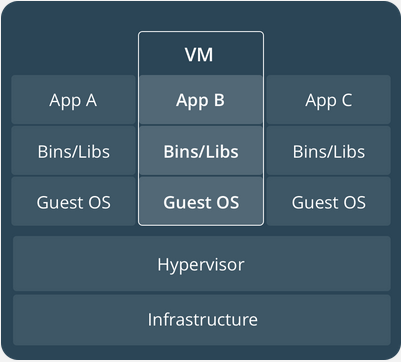
\includegraphics[width=0.495\textwidth]{img/Docker_VM.png}}{\caption{Virtual machine architecture, source \cite{Docker_docs}}\label{fig:Docker_VM}}
\ffigbox{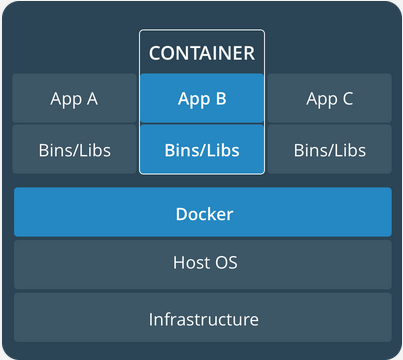
\includegraphics[width=0.5\textwidth]{img/Docker_container.png}}{\caption{Containers architecture, source \cite{Docker_docs}}\label{fig:Docker_container}}
\end{floatrow}
\end{figure}

\subsubsection{Virtual machine}
Let's start with a virtual machine (Fig. \ref{fig:Docker_VM}) and its layers description from the bottom up:
\begin{itemize}
\item \textit{Infrastructure} - It can be a PC, developer's laptop, a physical server in datacenter but as well a virtual private
server in the cloud as Microsoft Azure or Amazon EC2.
\item \textit{Host OS} - Host operating system. In case of native hypervisor this layer is missing. In case of hosted hypervisor
it is probably some distribution of Linux, Windows or MacOS.
\item \textit{Hypervisor} - Also called virtual machine monitor (VMM). It allows hosting several different virtual machines
on a single hardware. There are two types of hypervisors:
\begin{itemize}
\item Type 1 -  Also called \textit{bare metal} or \textit{native}. This type is run on the host's hardware to control it as well as manage 
the virtual machines on it. It is much faster and more efficient. This type hypervisors are KVM, Hyper-V or HyperKit.
\item Type 2 - So called \textit{embedded} or \textit{hosted} hypervisors. These hypervisors are run on a host OS as a software. They are slower
and less efficient on the other hand they are much easier to set up. It includes VirtualBox or VMWare Workstation.
\end{itemize}
\item \textit{Guest OS} - Guest operating system. Each VM requires own guest operating system which is controlled by the hypervisor. Each 
guest OS needs its own CPU and memory resources and starts on hundreds of megabytes in size.
\item \textit{Bins/Libs} - Each guest OS needs various binaries and libraries for running the application. It can be \textit{python-dev} or \textit{default-jdk} packages as well as personal packages to run the application.
\item \textit{Application} - The application source code that is desired to be run isolated. Therefore each application or each version of the application has to be run inside of its own guest OS with own copy of bins and libs. 
\end{itemize}

\subsubsection{Docker container}
\noindent
Now, what is different regarding containers (Fig. \ref{fig:Docker_container})
\begin{itemize}
\item \textit{Infrastructure} - PC, laptop, physical or virtual server.
\item \textit{Host OS with container support} - Any OS capable of run Docker. All major distributions of Linux are supported and there are ways
to run Docker even on MacOs and Windows too.
\item \textit{Docker engine} - Also called Docker daemon. It is a service that runs in the background on host operating system. It manages all interaction with containers.
\item \textit{Bins/Libs} - Binaries and libraries required by the application. They get built into special packages called \textit{Docker images}.
The Docker daemon runs those images.
\item \textit{Application} - Each application and its library dependencies get packed into the same Docker image. It is managed independently by the Docker daemon. 
\end{itemize}

\noindent
But the architecture is not the only one difference:
\begin{itemize}
\item Docker uses Docker daemon to manage containers, hypervisor manages virtual machines.
\item The Docker daemon communicates directly with host OS and manage resources for each container.
\item VMs usually boot up in a minute and more, containers start in seconds.
\item Docker virtualizes operating systems, using VMs is hardware virtualization.
\item VM and container vary in size. VMs start at hundreds of megabytes. A container can be smaller than one megabyte.
\item Containers share the kernel although they are isolated. VMs are monolithic and stand-alone.
\end{itemize}

\subsection{Dockerfile}
Dockerfile is a core file that contains the instruction to be performed when an image is built. It usually consists of commands to install packages, calls to other scripts, setting environmental variables, adding files or setting permissions. In Dockerfile there is also defined what image is to be used as a base image for the build.

\paragraph{Dockerfile instructions}
\begin{itemize}
\item \textit{FROM} - The FROM instruction defines the base image for next instructions and initializes a new build stage. Every Dockerfile
has to start with FROM command. The only exception is ARG command which can be before FROM command.
\item \textit{ARG} - The ARG instruction defines a variable that users can pass at build-time to the builder.
\item \textit{ENV <key>=<value>} - The ENV instruction sets the environment variables. It is key-pair value. 
\item \textit{LABEL} - The LABEL instruction adds metadata to an image. A LABEL is a key-value pair. It can be anything from version number to a description.
\item \textit{ADD <src> <dest>} - The ADD instruction copies files or directories from source and adds them at the destination path. It also unzips or untars files when added.
\item \textit{COPY <src> <dest>} - Similar to the ADD instruction it copies files or directories from source and adds them to the destination path. This command doesn't provide any kind of decompression.
\item \textit{RUN <command>} - The RUN instruction will execute any defined command and commit the results.
\item \textit{CMD ["executable","param1","param2"]} - The CMD instruction provides defaults for an executing container. It can include an
executable. In case the executable is omitted the CMD instruction must be used together with the ENTRYPOINT instruction. There can be only
one CMD instruction in Dockerfile. In case there is more CMD the last one will be used.
\item \textit{ENTRYPOINT} - The ENTRYPOINT defines a container configuration that will run as executable.
\item \textit{WORKDIR /path/to/dir} - The WORKDIR instruction sets the working directory for any RUN, CMD, COPY and ADD instruction that follows in Dockerfile.
\item \textit{EXPOSE} - The EXPOSE instruction informs Docker that the container listens on the specified network ports at runtime.
\item \textit{VOLUME} - The VOLUME instruction creates a mount point with the specified name and marks it as holding externally mounted volumes from the native host or other containers.
\end{itemize}

Except for the FROM instruction, all the instructions can be defined from the command line when starting docker container. There are more Dockerfile instructions however they are not relevant to this thesis as there are never used in practical part.
